\title{solution overview}
\begin{center}
\textbf{Chapter 03}\\
\vspace{2.5mm}
   \section{ \large \textbf{Solution Over View}}
\end{center}
\vspace{5.5mm}
    \subsection{Introduction}
    An employee management system is a comprehensive software solution designed to
streamline and automate various HR (Human Resources) processes within an organization.
It serves as a centralized platform to efficiently manage employee data, facilitate
communication, and optimize HR operations. The solution offers a wide range of features
tailored to meet the needs of HR professionals, managers, and employees, enhancing
productivity and promoting a positive work environment. Here is an overview of the key
features and benefits of an employee management system. Maintain detailed employee
profiles with personal information, contact details, work history, qualifications, and
performance records. Enable easy access to employee data for HR professionals and
managers. Automate attendance tracking, allowing employees to clock in and out
electronically. Streamline leave requests and approvals, ensuring accurate leave balances
and compliance with company policies. Conduct regular performance evaluations and track
employee progress. Set and monitor individual and team goals to align with organizational
objectives. Handle payroll processing, including salary calculations, tax deductions, and
benefit management. Ensure accurate and timely payment to employees. Facilitate internal
communication through messaging and chat features. Promote collaboration among
employees and between employees and management. Generate reports and analytics to gain
insights into workforce metrics, trends, and performance. Use data-driven decision-making
for talent management and strategic planning.
\newpage
\subsection{DFD -Data Flow Diagram}
A context level diagram is a type of Data Flow Diagram (DFD) that provides a high-
level overview of a system or process. It illustrates the interactions between the
system and its external entities, such as users, other systems, or organizations. The
context level diagram shows only one process, represented by a single bubble, and
the entities that interact with it, represented by rectangles.
\begin{figure}[h]
    \centering
    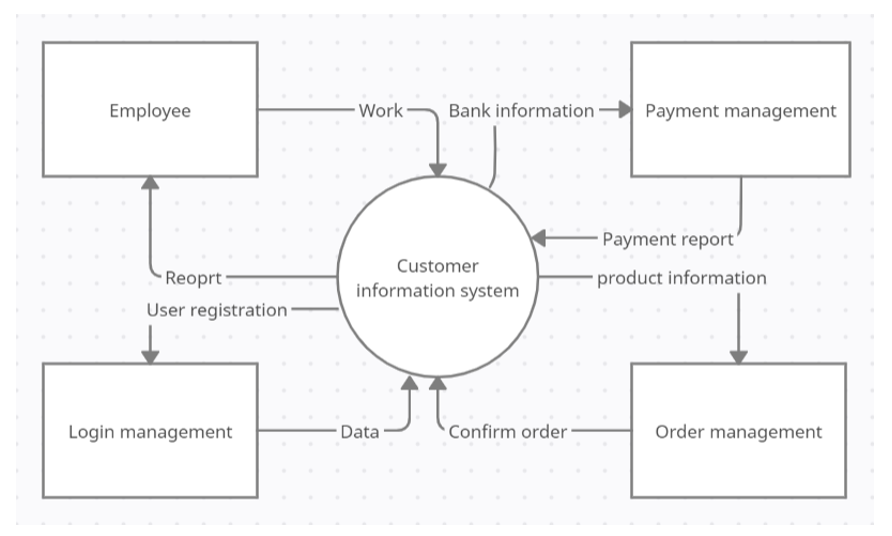
\includegraphics[height=8cm]{img/dfd.png}
    \caption{Data Flow Diagram}
    \label{fig:dfd}
\end{figure}
\newpage
\subsection{Use case Diagram}
A Use Case Diagram is a type of behavioral diagram in the Unified Modeling Language
(UML) used to visualize the functional requirements of a system from the perspective
of its users. It provides a high-level view of the interactions between users (actors)
and the system, depicting how users interact with the system to achieve specific goals
or tasks.
\begin{figure}[h]
    \centering
    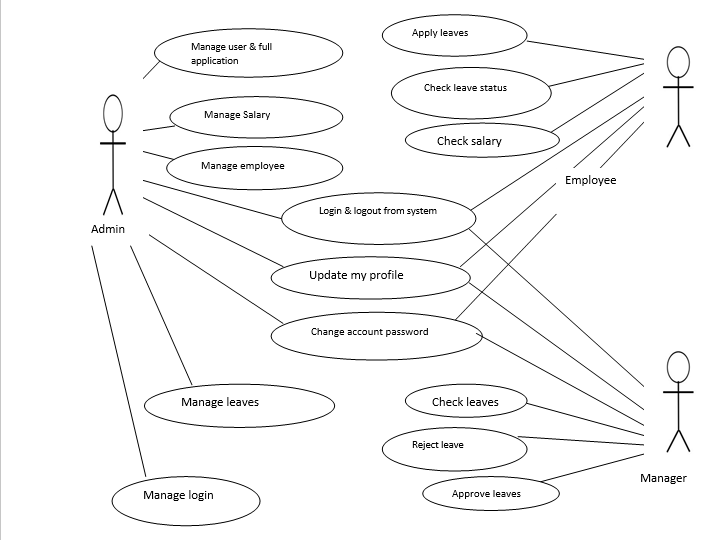
\includegraphics[height=8cm]{img/usecase.png}
    \caption{Use Case Diagram}
    \label{fig:enter-label}
\end{figure}
\newpage
\subsection{ER Diagram}
ER (Entity-Relationship) diagram is a graphical representation of entities and
their relationships in a database. It helps to model and design databases by
identifying the different types of data and relationships between them.
\begin{figure}[h]
    \centering
    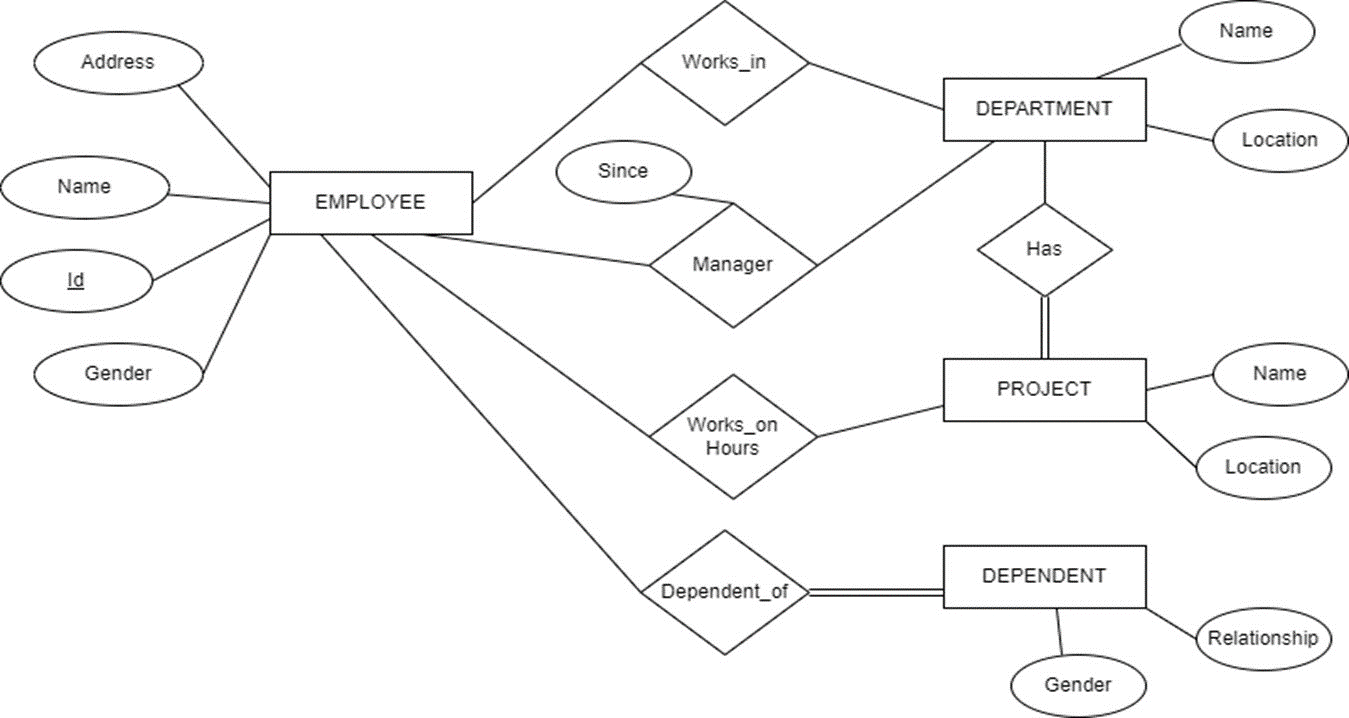
\includegraphics[height=8cm]{img/erdia.png}
    \caption{Entity-Relationship Diagram}
    \label{fig:erdiagram}
\end{figure}
\newpage
\subsection{Architecture Diagram}
\begin{figure}[h]
    \centering
    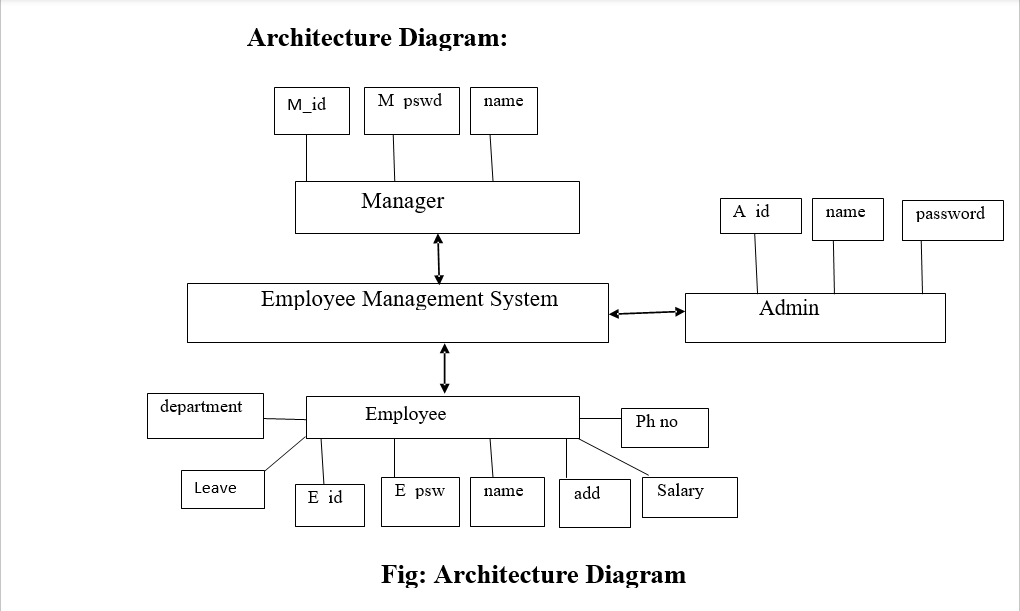
\includegraphics[height=8cm]{img/artich.png}
    \caption{Architecture Diagram}
    \label{fig:enter-label}
\end{figure}
\newpage
\subsection{Conclusion}

An employee management system is a powerful and indispensable solution that
revolutionizes the way organizations manage their workforce and HR processes. By
centralizing employee data, automating HR tasks, and fostering effective communication,
these systems significantly improve HR efficiency, employee engagement, and overall
business success. The comprehensive features offered by employee management systems,
such as employee profiles, attendance and leave management, performance evaluations,
payroll processing, training and development, and communication tools, create a cohesive
and productive work environment. Real-time reporting and analytics empower HR
professionals and managers with data-driven insights, enabling better decision-making and
talent management. The benefits of implementing an employee management system are
vast. Increased efficiency through automation reduces manual workload, enhances accuracy,
and minimizes errors. Employees benefit from transparent communication, performance
feedback, and training opportunities, leading to higher engagement and job satisfaction.
Additionally, compliance with labor laws and regulations is streamlined, and data security
ensures sensitive employee information remains protect.